\section{Componentes da DSL Cotas no \gls{MPS}}
\label{sec:mps}

Nessa Seção são descritos os elementos de modelagem criados na ferramenta \gls{MPS} tais como: os componentes de estrutura (\texttt{structure concepts}), a sintaxe dos editores projecionais (\texttt{editors}), restrições de escopo (\texttt{constraints}), comportamentos de conceitos (\texttt{behaviors}), sistema de tipos (\texttt{typesystem}) e, por fim, os elementos de geração de texto (\texttt{textGen}).

\subsection{\textit{Componentes de estrutura}}
\label{sub:sec:estrutura}

\textit{Concepts} ou conceitos no \gls{MPS} servem para definir a estrutura base da linguagem, cada conceito pode conter propriedades, outros conceitos filhos \texttt{childrens} e referências para outros conceitos. Eles podem herdar ou implementar características de outros conceitos. A Figura \ref{fig:structure} apresenta a lista de conceitos criados para a DSL Cotas.

\begin{figure}[ht!]
\centering

\caption{\textmd{Lista de Conceitos de Estrutura \gls{MPS}}}
\label{fig:structure}
\fcolorbox{gray}{white}{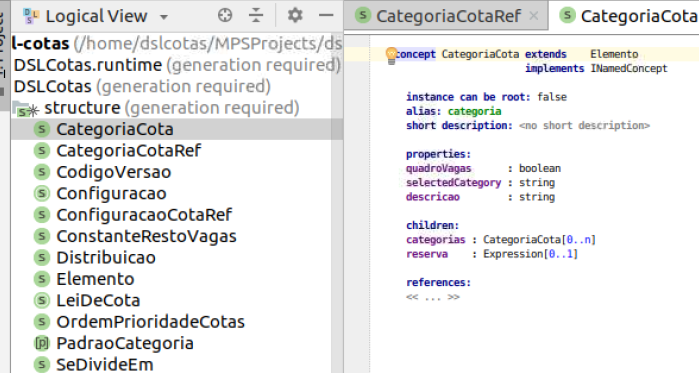
\includegraphics[width=0.70\textwidth]{chapters/dslcotas/mps/imagens/structure.png}}

\par\medskip\textbf{Fonte:} Elaboração do autor (2020) \par\medskip

\end{figure}





Esses conceitos definem a estrutura hierárquica da \gls{AST} de modo análogo ao modelo orientado a objetos, portanto, a Figura \ref{fig:classesmps} mostra a representação da modelagem dos conceitos em formato de diagrama de classes da \gls{UML}.

\begin{figure}[ht!]
\centering

\caption{\textmd{Modelo de Conceitos no \gls{MPS}}}
\label{fig:classesmps}
\fcolorbox{gray}{white}{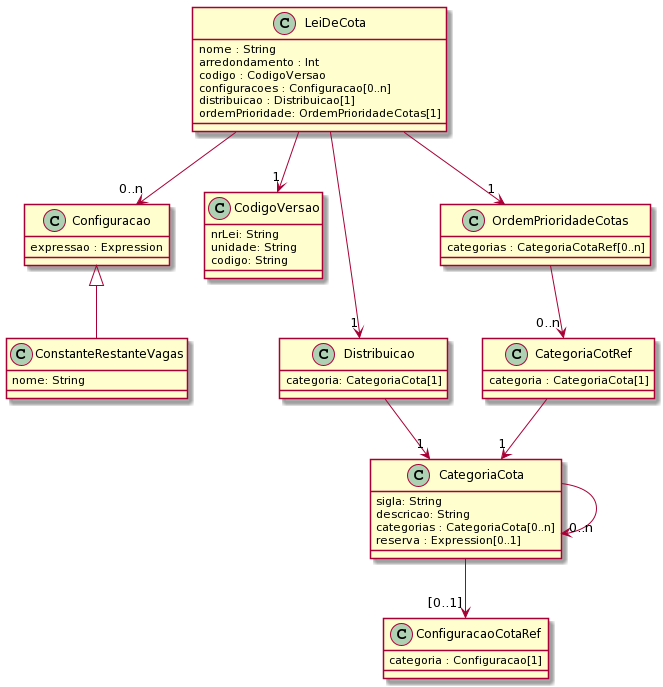
\includegraphics[width=0.70\textwidth]{chapters/dslcotas/mps/imagens/classesmps.png}}

\par\medskip\textbf{Fonte:} Elaborada pelo autor (2020). \par\medskip

\end{figure}




\newpage
O conceito \texttt{LeiDeCota} é o elemento raiz  que pode ser instanciado no \gls{MPS} a fim de criar uma representação abstrata de uma nova lei de cotas na DSL. No \gls{MPS}, os conceitos raiz podem ser criados em módulos \texttt{Solutions}, os quais utilizam uma ou mais linguagens e são os responsáveis por conter o código fonte do usuário final (Figura \ref{fig:solutions}).

\begin{figure}[ht!]
\centering

\caption{\textmd{Criação de elementos raiz em  \texttt{Solutions} no \gls{MPS}}}
\label{fig:solutions}
\fcolorbox{gray}{white}{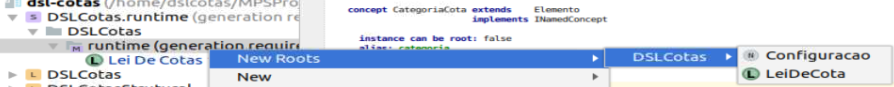
\includegraphics[width=\textwidth]{chapters/dslcotas/mps/imagens/solutions.png}}

\par\medskip\textbf{Fonte:} Elaboração do autor (2020) \par\medskip

\end{figure}



Por sua vez, uma \texttt{LeiDeCota} está associada aos elementos descritos na Tabela \ref{tblelementoslei}:

\begin{table}[ht]
\caption{Elementos associados ao conceito \texttt{LeiDeCota}}
\label{tblelementoslei}
\centering
\begin{tabular}{|p{4.2cm}|p{10cm}|}
\hline
\texttt{CodigoVersao}          & Elemento que mantém informações descritivas sobre a versão de lei aplicada.                                                                                           \\ \hline
Lista de \texttt{Configuracao} & Responsável por armazenar os parâmetros de configuração a serem reutilizados na DSL, contendo o nome da configuração e uma expressão de valor.                          \\ \hline
\texttt{Distribuicao}          & Conceito que contém a \texttt{CategoriaCota} raiz que dará início ao processo de distribuição das vagas entre as suas categorias filhas.                                       \\ \hline
\texttt{OrdemPrioridadeCotas}  & Elemento que contém a lista de referências para as categorias de cotas criadas durante a distribuição e será responsável por manter a ordem de prioridade prevista em lei. \\ \hline
\end{tabular}
  \par\medskip\textbf{Fonte:} Elaborada pelo autor (2020). \par\medskip
\end{table}

   
    

Para possibilitar a relação entre as regras definidas, alguns componentes da \gls{DSL} utilizam \texttt{references} para outros, possibilitando que elementos já definidos possam ser acessados pelos comandos \texttt{control+espaço} no \gls{MPS}. As \texttt{references} são restringidas pelo tipo do conceito alvo e pela cardinalidade, por exemplo, o conceito \texttt{CategoriaCotaRef} possui uma referência para uma \texttt{CategoriaCota} e, por sua vez, o elemento \texttt{OrdemPrioridadeCotas} possui lista de \texttt{CategoriaCotaRef} para que seja possível indicar na linguagem a ordem de prioridade criada durante a distribuição de vagas (Figura \ref{fig:references}).

\begin{figure}[ht!]
\centering

\caption{\textmd{Definição de \texttt{References} no \gls{MPS}}}
\label{fig:references}
\fcolorbox{gray}{white}{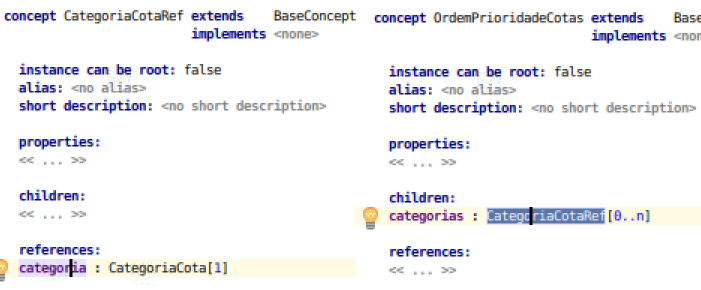
\includegraphics[width=\textwidth]{chapters/dslcotas/mps/imagens/references.png}}

\par\medskip\textbf{Fonte:} Elaborada pelo autor (2020). \par\medskip

\end{figure}



\newpage
Por fim, o conceito \texttt{Distribuicao} é o responsável por armazenar a árvore de distribuição, iniciando com a \texttt{CategoriaCota} raiz, na qual contém uma sigla, uma descrição, uma \texttt{Expression} onde será preenchida a reserva de vaga (percentuais fixos ou itens de \texttt{Configuracao} pré-definidos) e também uma lista de categorias filhas. 

Na Subseção \ref{sub:sec:editores}, serão apresentados os editores criados para definição da sintaxe de cada conceito definido na modelagem.


\subsection{\textit{Editores de conceitos}}
\label{sub:sec:editores}

\subsection{\textit{Restrições de escopo}}
\label{sub:sec:constraints}

\subsection{\textit{Comportamento dos elementos de conceito}}
\label{sub:sec:comportamentos}

\subsection{\textit{Sistema de tipos}}
\label{sub:sec:typesystem}

\subsection{\textit{Gerador textGen}}
\label{sub:sec:texgen}